%% MGT 6203 Progress Report: Group 95

\documentclass{article}
\usepackage[english]{babel}
\usepackage[utf8]{inputenc}
\usepackage{johd}
\usepackage{wrapfig}
\usepackage{tabularx}
\usepackage{enumitem}
\usepackage{hyperref}
\usepackage{amsmath}

%% ||| Title ||| %%
\title{MGT 6203 - Data Analytics for Business\\Final Report: Team 95}

%% ||| Authors ||| %%
\author{Daniel Forcade, Ryan Hopkins, Soheil Sameti, Steven Wasserman\\

}
%% ||| Date ||| %%
\date{April 21, 2024}

\begin{document}

\maketitle

%% ||| Github Link Embed ||| %%
\begin{center}
\textbf{Github: }{\url{https://github.gatech.edu/MGT-6203-Spring-2024-Canvas/Team-95 } }
\end{center}

%% ||| Section I : Background & Problem Statement ||| %%  [1]
\section{Background \& Problem  Statement}
\label{sec:background}
\hspace{.5cm} Weather plays a significant role in the cultivation of crops worldwide, as farmers rely on advantageous meteorological conditions to grow their crops. For years, farmers and agronomists alike have studied the weather to better understand its impacts on agricultural output, including temperature patterns, precipitation, extreme weather events, and more. The Old Farmer’s Almanac is a prime example – a comprehensive guide that recommends annual crop production periods, harvesting approaches, and more through the presentation of “astronomical data, reference charts, planting tables, weather forecasts, and more” \citep{FineGardening}.

Modern approaches to optimizing output rely on a set of practices known as precision agriculture, defined as the process of analyzing “temporal, spatial and individual plant… to support management decisions according to estimated variability for improved resource use efficiency, productivity, quality, profitability and sustainability of agricultural production” \citep{ISPA}. The collection and analysis of data to support such decision-making can illuminate dynamic weather events and processes that affect different stages of plant growth including soil erosion, nutrient deficiency, and, in cases of drought, soil salinization \citep{EOS}.

Extensive climate information at a regional level is made available to farmers through governmental organizations, similar to how you receive weather updates from your local news station. Known as a "local extension agencies," these offices offer valuable information and learning engagements for farmers, including weather and climate reports. These reports, however, cannot effectively appraise weather conditions at a level localized to individual farms or sections of a farm - think of getting a weather forecast for your home's address. The micro-climate conditions of these areas might differ significantly from regional climate forecasts, necessitating different farming practices and approaches to achieve greater success. And while farmers can collect weather data using common instruments, like affixed weather sensors that come standard with John Deere tractors \citep{JohnDeere}, functional models that take in such data and produce effectual insights are not readily available to farmers. 

\begin{wrapfigure}{r}{0.5\textwidth}
  \begin{center}
    \vspace*{-5mm}
    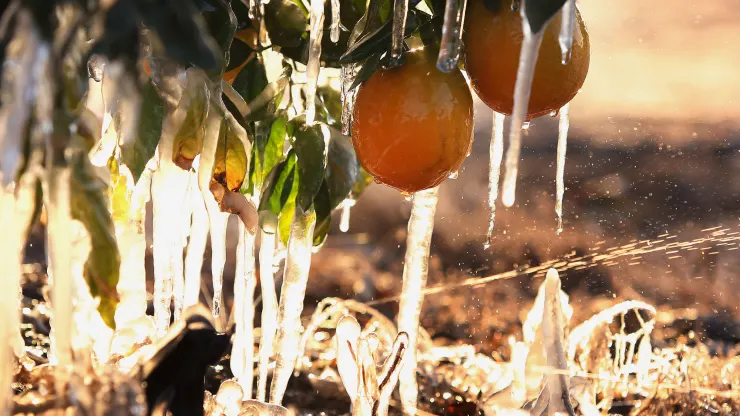
\includegraphics[width=0.45\textwidth]{Final_Report/images/frozen_oranges.jpeg}
  \end{center}
  \vspace*{-5mm}\caption{Frozen oranges during a cold snap in December 2013 affecting the San Joaquin Valley citrus crop, in Traver, CA \citep{Orange}}
\end{wrapfigure}

This persistent issue draws an impactful business case for further research and is the topic of focus in this paper. Especially as climate change becomes more of a heightened uncertainty for the global economy, studying the effects of micro-climate weather effects on crop cultivation can aid in recommending crop growth practices to farmers and supporting the industry in sustaining resilient crop markets.

Understanding the impacts of local climate conditions at the farm level can be used to propose remediation tactics for farmers before disaster strikes. Bad weather can greatly impact the business of farming, leading to huge losses and productivity fallout. For example, seven days of freezing temperatures in 2013 led to the loss of 200,000 acres of citrus groves in California, resulting in damages amounting to \$2 billion \citep{CNBC}.

This research project aims to determine the efficacy with which localized micro-climate conditions can recommend crop production. The research will illuminate the correlation between climate conditions and crop yields for specified locations across California. The research will further demonstrate a proof-of-concept tool that can apprise farmers of impending risks to their crops based on micro-climate conditions and recommend crops to plant and harvest based on these risk factors as well as historical and predicted climate conditions. 

%% ||| Section II : Approach ||| %%  [2]
\section{Approach}\label{sec:approach}
\hspace{.5cm}The research project looks to analyze the climate conditions and crop yields of specified locations in the United States to identify relationships between localized weather patterns and crop yields that can be used to recommend crop production based on changing climate conditions. The research will focus on, at most, two locations of interest to validate whether the methodology is repeatable across disparate locations. Data curation will entail the collection of local-level weather data and crop production data, either at the county or ZIP code level as available. Next, data will be joined based on geospatial coordinate systems to align crop yield to direct weather conditions. Model generation will include a cadre of statistical methods, including regression to analyze cardinal temperature effects on crop production, clustering and classification to group weather conditions to crops, and cumulative sum approaches to detail weather condition changes on crop production. 

While similar approaches, such as those outlined by \citet{UIUC} and \citet{ISWS}, have performed analyses of crop production based on regional weather conditions, those researchers did not recommend approaches for using modeling with micro-climate conditions and maintained greater geographic areas of observation with their approaches. Our approach looks to collect weather data at the county or ZIP code level and relate that to crop production at the same level of observation, rather than a state or state-regional level. \citet{RemoteSens} used geospatial heatmaps of American topography to assess crop growth conditions at a county scale. Our research will operate in a similar vein, using locally measured temperature data instead of satellite infrared photography. Our approach is similar to that of \citet{Sustainability}, where several climate metrics were assessed across the Naoli River Basin in Northeast China to determine the suitability of crop production for a variety of plants. Our research, however, will not consider human factors like \citet{Sustainability} and focus exclusively on weather conditions, as it is assumed the intended users of such models would be comprised of local growers and farmers who are intimately aware of their farm's growing practices. This audience would need to be informed of approaches to incorporating insights from this research to create micro-climate models for weather conditions. A secondary audience could include federal lawmakers and employees who support federal incentives and harvest programs that can affect market conditions and promote the cultivation of specified crops. In dissenting from \citet{Sustainability}, our research would assume that human-driven decision-making could be influenced by such federal programs and market incentives. 

% This research, however, will not consider human factors, which drive the conversation of the intended audience for this research. Our team would look to promote the outcomes of this research to federal lawmakers and employees who support federal incentives and harvest programs that can affect market conditions and promote the cultivation of specified crops. For this research, then, the team will assume that human-driven decision-making could be influenced by such federal programs and market incentives. 

It should be noted that data-driven analyses such as this one are typically performed by academic institutions and corporations with the funds and resources to carry out large projects. By codifying this approach and describing the intended audience, the team looks to federate information to those without such resources and empower local growers and farmers to use this information to benefit their farming practices and respective businesses. 

%% ||| Section III : Data ||| %%  [3]
\section{Data}
\hspace{.5cm}For this research effort, the process of identifying, processing, curating, and saving data is described to illuminate identified data sources, challenges with data, and key information. The data needed to support the outlined research questions includes localized weather data and localized crop yield data. The team decided to use California and Florida as test cases for the research project, given the diversity of weather patterns that occur throughout these large states. However, Vermont and Iowa were initially used to parse data from sources given their relative observed simplicity, and data was collected for these states as well. Artifacts of these states might appear in developed code. 

\subsection{Data Discovery}
\hspace{.5cm}The data needed to support the research includes localized weather data and localized crop yield data. The team reviewed several different resources online for both data domains, looking to find widely available, well-populated sources that would have the information that could best meet our needs. The primary sources the team identified and decided to use for the research are:
\begin{itemize}
    \item The USDA National Agricultural Statistics Service (NASS) Cropland Data Layer (CDL) is "an annual raster, geo-referenced, crop-specific land cover data layer produced using satellite imagery and extensive agricultural ground reference data" \citep{NASS-CDL}.
    \item The Global Surface Summary of Day (GSOD) dataset describes surface summary weather conditions, such as temperature and wind speed, for 9000 global weather stations \citep{NOAA-NCEI}. The NCEI is an office of the National Oceanic and Atmospheric Administration (NOAA).
    \item The National Climate Data Center (NCDC) Storm Events Data describes personal injuries, data estimates, and related storms recorded by county in the United States since 1950 \citep{NOAA-NCDC}. The NCDC is the world's largest climate data repository, located in Asheville, NC, and owned and operated by the National Oceanic and Atmospheric Administration (NOAA).
\end{itemize}

Crop data was initially found using George Mason University's \href{https://nassgeodata.gmu.edu/CropScape/}{CropScape} tool, an interactive GUI that shows crop yields for different counties across the United States. The GMU tool sources its data from the NASS Cropland Layer Data source that was ultimately selected. 

\subsection{Data Preparation}

\begin{wrapfigure}{l}{0.5\textwidth}
  \begin{center}
    \label{sec:raster}
    \vspace*{-8mm}
    \includegraphics[width=0.45\textwidth]{Final_Report/images/raster_example.jpeg}
  \end{center}
  \vspace*{-5mm}
  \caption{Rendered raster image representing Carroll County in the State of Iowa, U.S. \citep{RemoteSens}}
  \vspace*{-2mm}
\end{wrapfigure}

\hspace{.5cm}After identifying each of the data sources, several preprocessing and cleaning procedures were completed to convert the data to a usable format. The datasets contained geographic location components that were in various spatial formats that could not be directly linked for analysis.  To address this, we implemented a geographic conversion and standardization pipeline that is detailed below.

The Cropland Layer Data (CDL) included crop yield for different regions using raster data, which is a gridded, pixelated data format typically associated with an identified geographical region as shown in \textbf{\hyperref[sec:raster]{Figure 2}}. This raster data was saved using Tag Image File Format (TIFF) files, the standard for storing raster image information, with each observation representing 0.22 acres of land. The raster files are compatible with ArcGIS but ill-suited for vector dataframe analysis. To solve this problem, we implemented a raster-to-vector converter utilizing \texttt{Rasterio} in Python with a EPSG:4326 geographic coordinate system. Our conversion pipeline takes in the CDL raster files for a given U.S. state, creates a descriptor column for the crop type, and then refactors the EPSG:4326 spatial data into the latitude/longitude coordinates of each observation. 

The data from the conversion pipeline resulted in massive vector files that needed to be condensed. To solve this, we created a secondary pipeline that used spatial joins with additional shapefiles from the U.S. Census (\citeyear{TIGER}) to generate regions of interest that could be more easily matched to the weather station data. Each crop was grouped and aggregated into a summarized region, such as county or ZIP code, which significantly compressed the crop data into a manageable format for tabular analysis. This second pipeline also appended additional information from the U.S. Census data, namely land area and water area. The weather datasets initially included latitude/longitude data for each observation, which made it convenient to link to the modified crop data. Using the U.S. Census data, each weather station was matched to the regions of interest defined in the crop data. 

Data validation measures were taken to ensure that the data was clean and resolute. Using data documentation from the sources, encoding was used to replace N/A values with missing flags (e.g., \texttt{-999.99} in weather) as well as reverse-encoding binary string signifiers for weather events (e.g., \texttt{01001} into "Rain and Wind"). 

Several issues arose in carrying out the data cleaning. Memory allocation issues arose with using R to perform the CDL raster conversion. The code was modified to use resolution reduction and batched parallel processing, but did not work. Instead, Python was used successfully. Another issue arose with using the Google Maps API and R package \texttt{zipcodeR} to determine a regional descriptor for each latitude/longitude observation, such as ZIP code or county. While the script worked on sample datasets, scaling up the data resulted in a slower program that could not work efficiently.

Subsets of the processed crop data and weather conditions data for California can be seen in \textbf{\hyperref[sec:cropsubset]{Figure 3}} and \textbf{\hyperref[sec:weathersubset]{Figure 4}}. Additional data elements were joined and are available for analysis, including dew point, wind gust, and more, as described in \textbf{\hyperref[sec:curated]{the appendix}}. \\

\begin{figure}[H]
\vspace*{-5mm}
\label{sec:cropsubset}
\centering
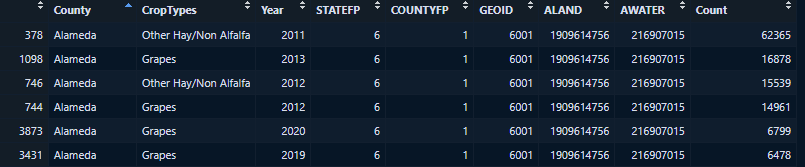
\includegraphics[width=1.0\textwidth]{Final_Report/images/Crop_Dataset.png}
\vspace*{-5mm}
\caption{Subset of crop data for California}
\end{figure}

\begin{figure}[H]
\vspace*{-5mm}
\label{sec:weathersubset}
\centering
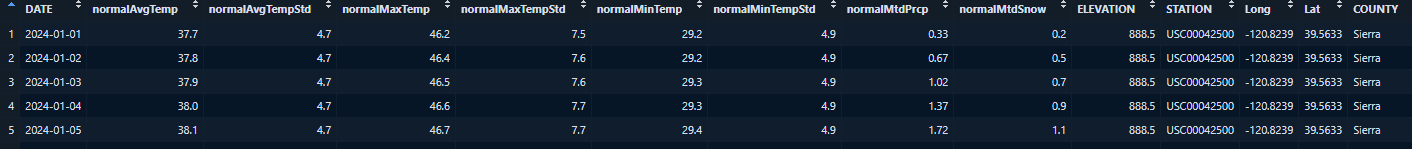
\includegraphics[width=1.0\textwidth]{Final_Report/images/Normals_Dataset.png}
\vspace*{-5mm}
\caption{Subset of 30-yr. temperature normals for California}
\end{figure} 

\subsection{Advanced Data Manipulation}
\begin{wrapfigure}{r}[0pt]{0.4\textwidth}
  \vspace{-10pt} % Adjust vertical space before the figure
  \centering
  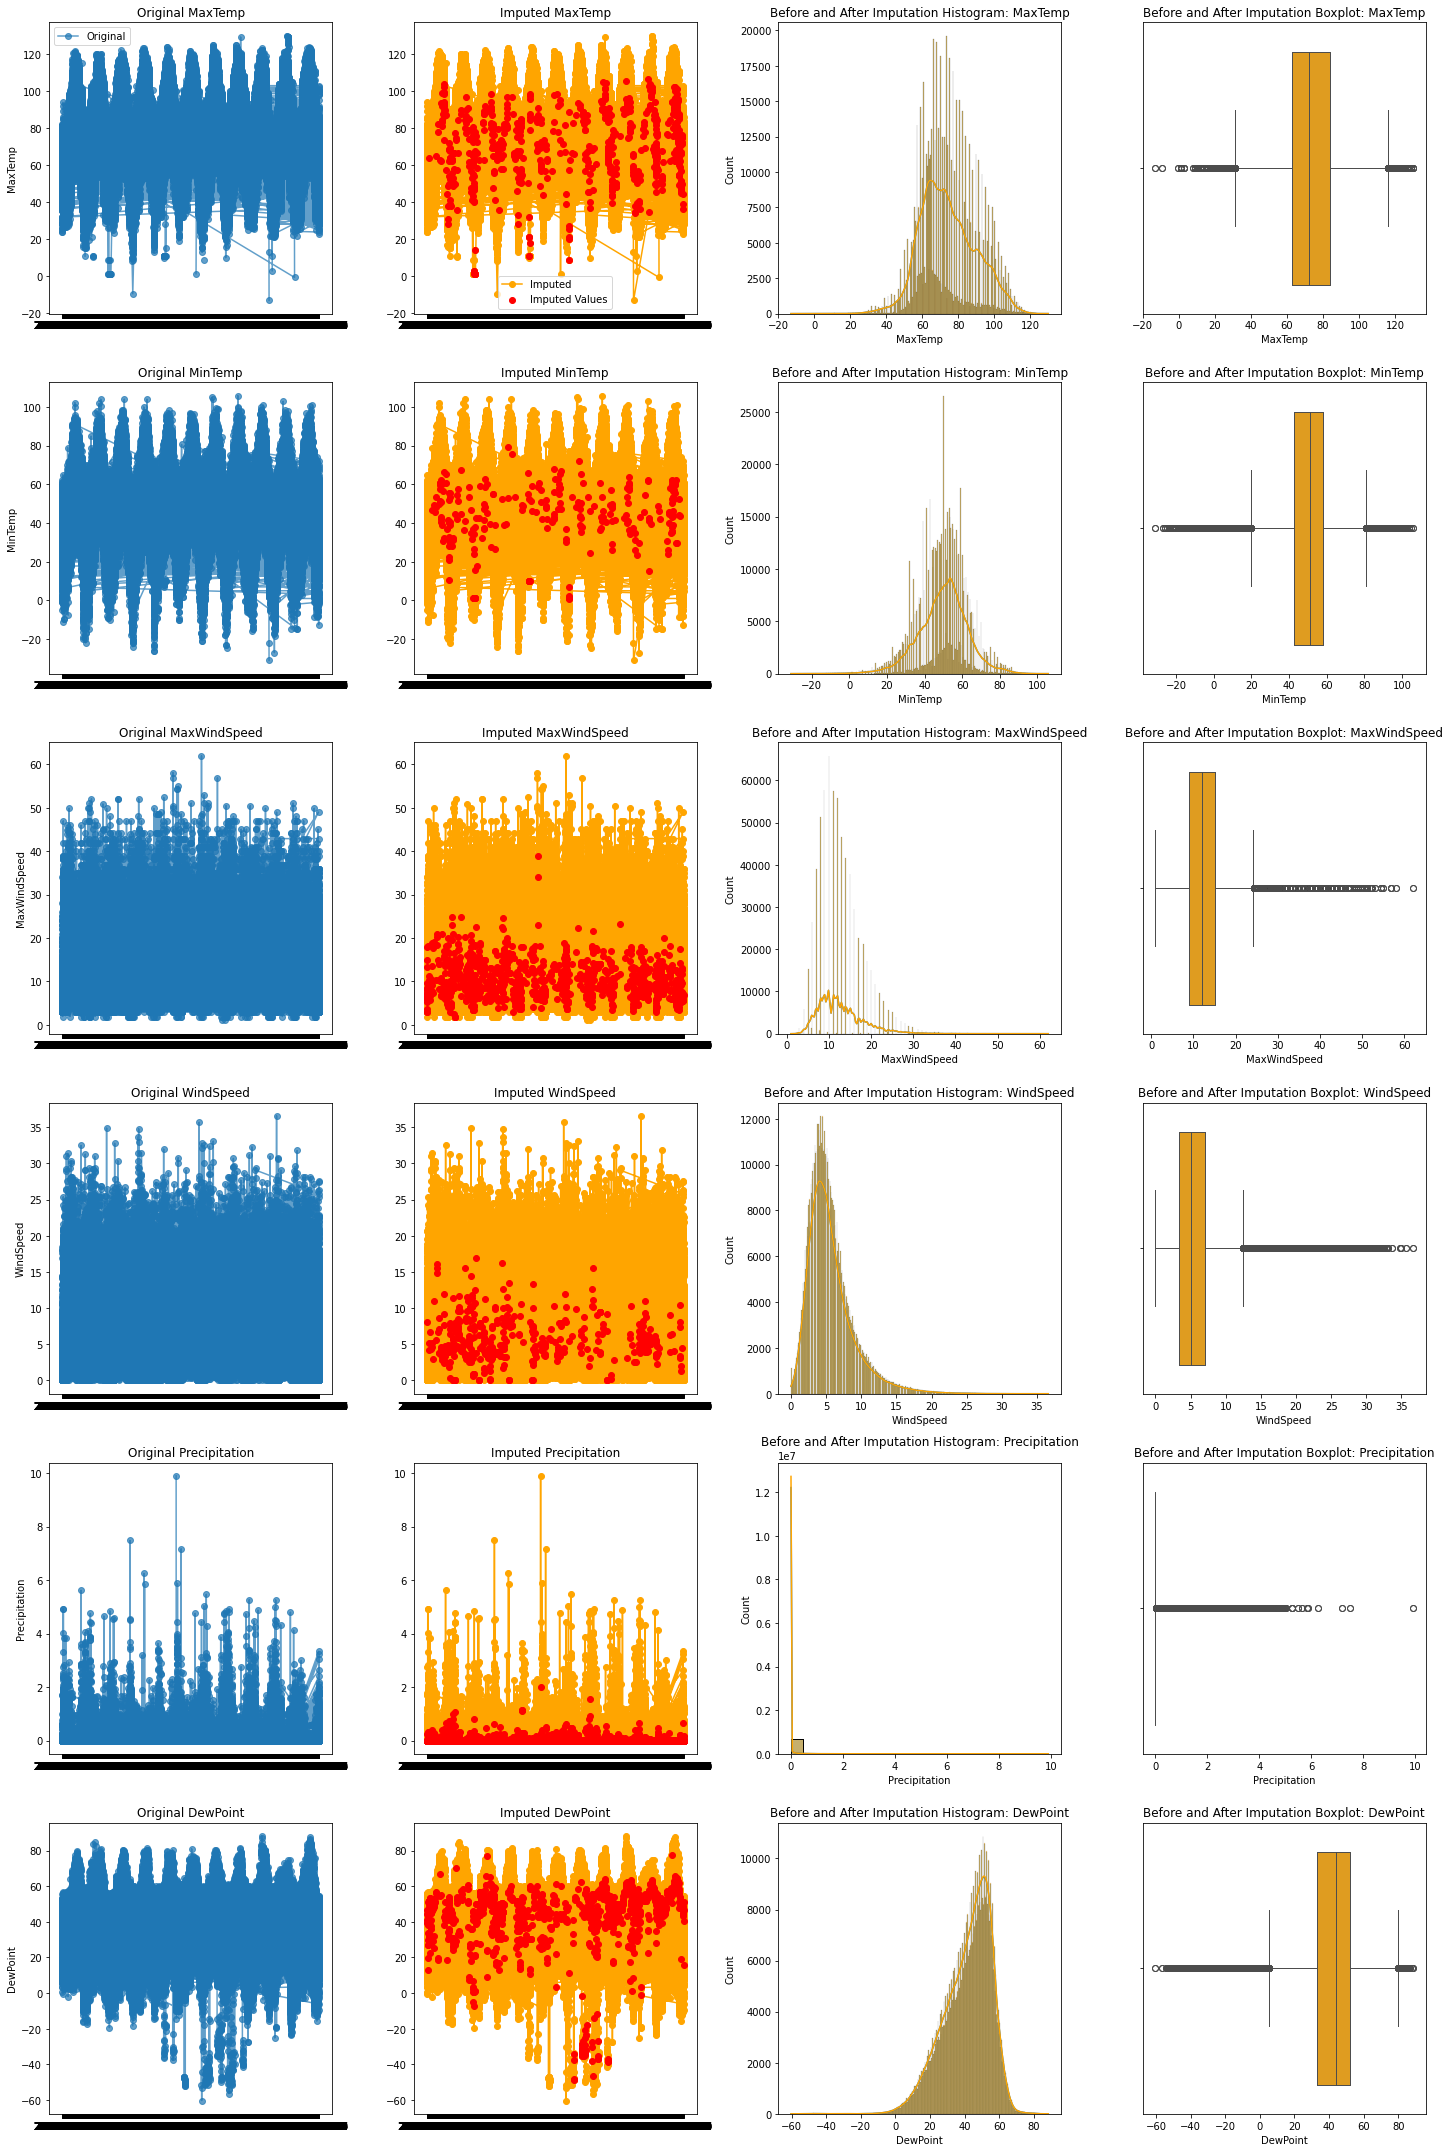
\includegraphics[width=0.4\textwidth]{Final_Report/images/Missing_Values_Imputation.png}
  \centering
  \caption{Imputation Analysis }
  \label{sec:Imputation Analysis}
  \vspace{-2pt} % Adjust vertical space after the figure
\end{wrapfigure}
\hspace{.5cm}While some basic data cleaning and preparation was performed preciously, more work was needed to finalize representative datasets appropriately. Of greatest concern was the daily weather dataset, which maintained a mixture of sporadic and block forms of missing data. Some of this data was classified as missing completely at random (MCAR), while others were not random at all - likely due to specific weather stations going offline for repairs or maintenance for extended periods of time. In one specific instance, weather stations reporting from Mexico did not have a defined U.S. county - understandable, but still noticeable in our analysis.

A series of matrix and heat-map plots were created in addition to summary statistics to visualize and quantify the nature of the missing data, then decided that a rolling-mean imputation would effectively preserve the structure of our data while creating minimal bias and disruption. A 6-day centered rolling mean was applied to key variables of interest, such as daily temperature, wind gust, and precipitation.

To validate the imputation, original and imputed data points were plotted to visually inspect the effectiveness of our imputation strategy. This included generating line plots to compare original and imputed values and highlighting imputed points in different colors to discern the character of the imputed values against the actual data trend. To further assess the impact of imputation on the data distribution, histograms, and box plots were generated to display pre- and post-imputation scenarios. This helped to evaluate whether the imputation method had unduly influenced the statistical properties of the dataset, such as mean, variance, and distribution shape.

In other instances, metrics between datasets were not standardized and needed to be the same unit to have an appropriate analysis. With the \hyperref[sec:spatial]{spatial analysis}, the units varied between datasets, including inches and millimeters (mm) of rain as well as acres, sq. miles, and sq. meters of farmland. These units were standardized for later analysis. 

Previously, the team used U.S. Census shape-files to map crop production and weather stations to county locations. While this information was useful in the context of preliminary analysis, it was not ideal in generating specific locations for later analyses, as counties are administrative in nature and not specifically designed with climate considerations. Moreover, in most cases, the weather stations that reported daily weather observations differed from weather stations that reported for the 30-year weather normals. To create a more refined and accurate climate pipeline, a nearest-neighbor spatial join was generated to link all location data together. Specifically:

\begin{itemize}[noitemsep]
    \item[-] Set daily weather stations as the primary anchor point.
    \item[-] Perform a nearest-neighbor spatial search to determine the nearest station reporting climate-normals for each station reporting daily observations.
    \item[-] Validate and search for extreme distances or anomalies in the nearest-neighbor spatial join by looking for distance outliers as well as create a visual identification plot.
    \item[-] Create a composite key on the nearest-neighbor results and perform a merge between daily weather records and 30-year climate normals.
    \item[-] Perform a nearest-neighbor spatial search to map crops to their nearest station reporting daily observations.
\end{itemize}

In this process, the team was able to create a robust spatial and temporal link between the three core data sources: Daily Weather Observations, 30-Year Climate Normals, and Crops. This was a crucial step, as recommendation or risk involving the weather requires as much as localized precision as possible.

%% !!!!!! Nearest Neighbors Plot !!!!! %%
\begin{figure}[H]
\vspace*{3mm}
\centering
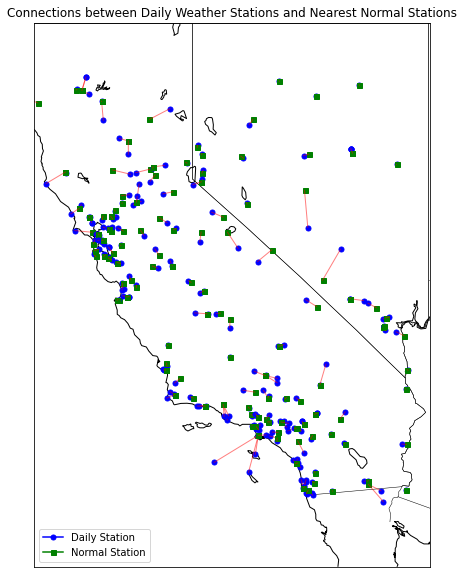
\includegraphics[width=0.55\textwidth]{Final_Report/images/Nearest_Neighbor_Stations_Mapping_Plot.png}
\vspace*{-5mm}
\caption{Nearest-Neighbor Clustering of Stations in CA}
\label{sec:Nearest Neighbors}
\end{figure}

\subsection{Data Curation}
\hspace{.5cm}From the result set of data that was prepared, the team distilled and curated the datasets down further to better later facilitate model development. For the crop production data, the team decided to focus on the top ten most valuable crops produced in California as part of the analysis. While the entirety of crops produced in CA could have been kept, focusing on the top ten provides sufficient scope, simplifies analysis, and maintains the underlying intent of the research to target commonplace farming practices (which necessitates targeting the most abundant crops produced in a given state and avoiding specialty crops). To accomplish this, the team used publications from the California Department of Food \& Agriculture (\citeyear{CA-Ag}) to define a list of the top ten crops produced by agricultural value. This list was compared with independent sources, including \citep{Stacker}, \citep{FGS}, and \citep{FarmingWork.com}, to validate that it was accurate and widely accepted. Filters were applied in R using observations on the representational descriptor variables, then data was split and saved. The selected crops for California are available in \textbf{\hyperref[sec:choices]{the appendix}}.

Once set, the team stored the data as CSVs into a shared folder hosted on the web in \href{https://gtvault.sharepoint.com/:f:/s/MGT-6203Team95/Ev1dI-WU521EnSnFGUY9QigBHe4nMzpq5NIJo9s6VWLIoA?e=qEVO1C}{SharePoint}. These datasets can be easily queried for further development later in the project, and describe the data necessary to answer the outlined research questions. Descriptions of the available data can be reviewed in \textbf{\hyperref[sec:curated]{the appendix}}.


%% ||| Section IV : Model & Analysis ||| %%  [4]
\section{Models \& Analysis}
\label{sec:ma}
Several different analyses were undertaken to evaluate the use of micro-climate data for crop yield recommendation. Three main analyses were performed, including:
\begin{itemize}[noitemsep]
    \item[1.] ArcGIS Suitability Analysis
    \item[2.] County Weather Condition Spatial Analysis for Crop Production Recommendation
    \item[3.] Crop Cultivation Risk Index Development
\end{itemize}

\subsection{ArcGIS Suitability Analysis} 
\label{sec:suitability} 

\begin{wrapfigure}{l}[0pt]{0.4\textwidth}
  \vspace{-10pt} % Adjust vertical space before the figure
  \centering
  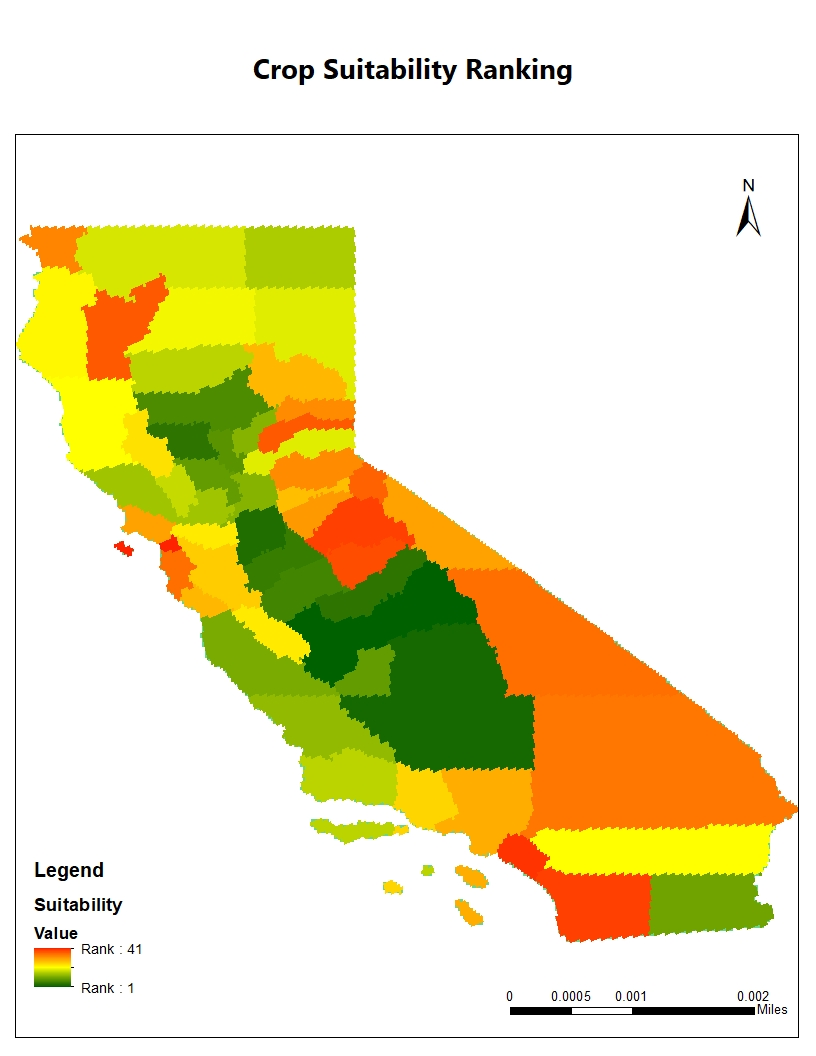
\includegraphics[width=0.4\textwidth]{Final_Report/images/Crop Suitability Ranking.jpg}
  \centering
  \caption{Crop Suitability Ranking for each County in CA}
  \label{sec:SuitabilityAnalysis}
  \vspace{-2pt} % Adjust vertical space after the figure
\end{wrapfigure}

\hspace{.5cm}The suitability analysis involves ranking the cultivation of each crop in each county by computing each crop's annual harvest in each county. This required reducing the dataset down to each crop's identified growing period, by using the cardinal weather data available, then computing its harvest in each county. Additionally, each county was then ranked by the total number of days crops can be produced. Therefore, each county receives two ranks: one for the amount of crops produced and the other for the total days that crops can be farmed.

The Weighted Overlay tool in ArcMap was then used to assign weights to each county. A maximum weighting of 70 was established as a maximum threshold for the amount of crops produced by each county. A minimum weighting of 30 was placed on the weather suitability ranking of the crops. Through this, the team assumed that areas with better infrastructure and experience are more suitable for crops. As shown in \textbf{\hyperref[sec:SuitabilityAnalysis]{Figure 7}}, certain counties in California are more adept at crop production based on a variety of factors and should be targeted as such. In the \textbf{\hyperref[sec:spatial]{following section}}, this idea is explored further through the creation of a ranking that deterministically broadcasts which crops should be produced in which counties based on localized climate conditions. 

Further work in this field could include additional commercial metrics for each county to underpin the ranking of counties, including influential factors like proximity, land value, topology, and profitability.

\subsection{County Weather Condition Spatial Analysis for Crop Production Recommendation}
\label{sec:spatial}
\hspace{.5cm}A spatial analysis is conducted to determine the current production totals of crops in each county of California, then recommend ideal counties for producing crops in the future through the use of cardinal temperatures and precipitation conditions data as well as spatial analysis of 10-year and 30-year climate normals. This analysis requires aggregation of different datasets to prepare the observed weather data for each county. The data is collated to find temperature and precipitation averages for each crop, then spatial analysis is used to compare each crop's cardinal climate attributes to the observed weather patterns in each California county. A ranking is produced that suggests, according to observed weather patterns, which crop each county should be producing. This is then compared to actual current production, a similar ranking of current crop production found in the \hyperref[sec:suitability]{suitability analysis}, to finalize a recommendation that suggests:
- Which crops each county in California should be producing based on observed weather conditions, including temperature and rainfall, from 2010-2020
- Which counties are currently producing according to model expectations, and which are not

While the code itself accepts a variable input for the top number of counties to compare, the top three counties were used for initial observation. Further, two sub-analyses are conducted, one that compares the use of 10-year climate normals to 30-year climate normals and the other that removes counties from analysis that do not fall within the range of minimum or maximum temperature and precipitation guidelines outlined by the cardinal climate conditions for the selected crops. These four subsets did not find a significant result, with less than 10\% of recommended counties matching the current counties that produce the top 10 most valuable crops in California. 

An emergent pattern of more matches could be observed if the \textbf{top-X} value was increased, but it is most likely due to data not in scope for this project. The next steps could seek to increase the fidelity of current data or identify new data that could describe the difference. 

Further, later work in this area could analyze soil composition and insect invasion patterns to further inform the given recommendations. Codifying the cyclical nature of annual pest invasion cycles could prove valuable to farmers to protect harvests through preventative measures. The inclusion of soil composition data could lead to more bountiful harvests, more sustained success, and greater individual outcomes for farmers. 

\subsection{Crop Cultivation Risk Index}
\label{sec:riskindex}
\hspace{.5cm}The most impactful component of this research included the creation of a Risk Index that employed two separate methods: binary and dynamic statistical threshold analysis. The end goal of this risk model is to synthesize all collated data, including daily weather observations, 30-year climate normals, crop production locations, and crop cardinal temperature conditions, into a generalized output that can be utilized to recommend crop production and alert on impending weather events for small-scale farmers and consumers based on their micro-climate patterns.

To create the Index, the team first designed a Binary Threshold, which prioritized categorizing temperature data into distinct binary states based on the daily temperatures, normal temperatures, and cardinal crop attributes for each unique daily station. We generated twenty-seven output variables of high and low thresholds for various temperature metrics and tracked whether they were above, below, or within acceptable ranges for each crop throughout the year, on a daily scale. These results were then aggregated into monthly totals, and a composite score was generated to assess risk. In \textbf{\hyperref[fig:left]{Figure 8}}, we demonstrate how this threshold method captures the amount of days within optimal growth ranges for various crops in a randomly selected station. In \textbf{\hyperref[fig:right]{Figure 9}}, we show a heat-critical graph for the same station; this is where the daily temperature average was above the absolute maximum temperature each plant could withstand. This method and model produced insight into the temporal and seasonal nature of our data, but did not quite capture the nuance required in terms of precision and scaling - it was primarily used to inform decisions for the Dynamic Statistical Threshold and associated index.

\begin{figure}[H]
  \centering
  % Left figure
  \begin{minipage}{0.48\textwidth}
    \centering
    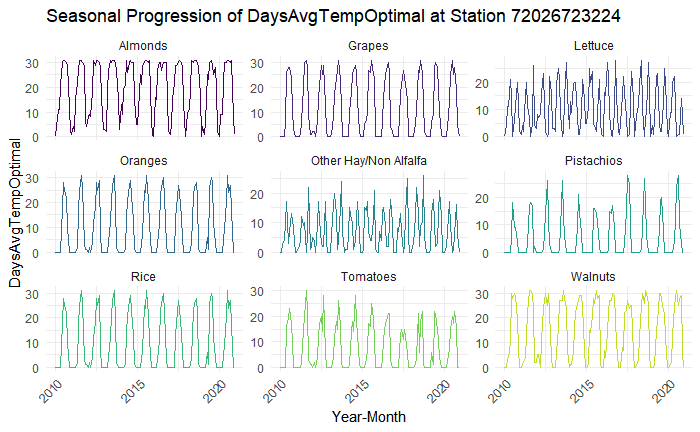
\includegraphics[width=\linewidth]{Final_Report/images/Index_Binary_Within_Optimal.png}
    \caption{Binary Threshold: Optimal Growth Days}
    \label{fig:left}
  \end{minipage}\hfill % Add some horizontal space between the figures
  % Right figure
  \begin{minipage}{0.48\textwidth}
    \centering
    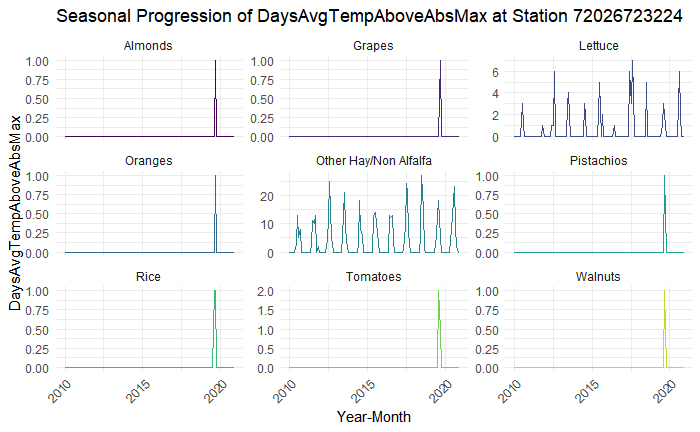
\includegraphics[width=\linewidth]{Final_Report/images/Index_Binary_Heat_Critical.png}
    \caption{Binary Threshold: Critical Days (Days AVG. Temp is above ABS Max)}
    \label{fig:right}
  \end{minipage}
\end{figure}

We developed the Dynamic Risk Index based on the foundation of the Binary Risk Index. For each day,the deviation of observed temperatures was computed from both the crop-specific cardinal temperatures and the statistical thresholds. This process identifies how often and to what degree temperatures fall outside optimal and absolute ranges for each crop. The model takes into account various weights such as the number of crops grown in the station region, the deviation above or below the optimal, the daily deviation compared to the 30 year normal of the region, and each plants specific tolerance for heat or cold. These scores and deviations are totaled into a dynamic risk index, which we have converted to a dashboard that can show which areas are most at risk for damage based on their temperature trends, historical weather, specific crops being grown, and amount of that crop being grown in that area.  We believe that with further refinement, there is a serious business use case for this type of localized recommendation and warning service in the market, especially with small scale farming.  We have set up preliminary Random Forest models assist with further refinement of our Index.

\begin{align}
\text{ScaledColdOptDeviation} &= \text{WeightedColdOptDeviation} \cdot \log_1p(\text{Count})^2 \cdot \text{CountWeight}, \\
\text{ScaledHeatOptDeviation} &= \text{WeightedHeatOptDeviation} \cdot \log_1p(\text{Count})^2 \cdot \text{CountWeight}, \\
\text{ScaledColdAbsDeviation} &= \text{WeightedColdAbsDeviation} \cdot \log_1p(\text{Count})^2 \cdot \text{CountWeight}, \\
\text{ScaledHeatAbsDeviation} &= \text{WeightedHeatAbsDeviation} \cdot \log_1p(\text{Count})^2 \cdot \text{CountWeight},
\end{align}

\begin{equation}
\begin{split}
\text{TotalRiskIndex} = & \ \text{ScaledColdOptDeviation} + \text{ScaledHeatOptDeviation} + \\
                        & \ \text{ScaledColdAbsDeviation} + \text{ScaledHeatAbsDeviation}
\end{split}
\end{equation}

%% !!!!!! Risk Dashboard !!!!! %%
\begin{figure}[H]
\vspace*{2mm}
\label{sec:Risk Dashboard}
\centering
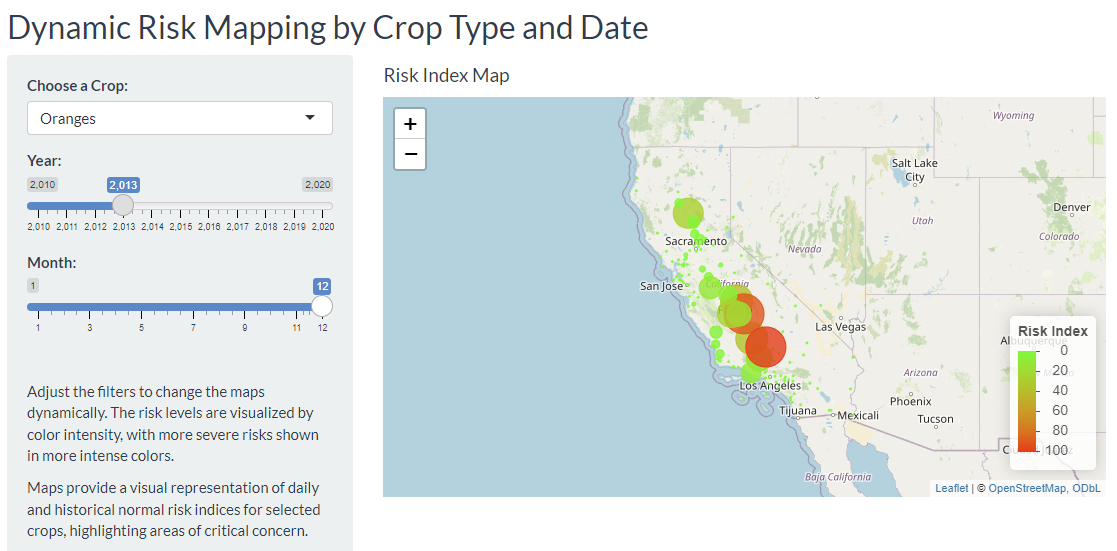
\includegraphics[width=.8\textwidth]{Final_Report/images/DynamicRiskIndex_Dashboard.png}
\vspace*{2mm}
\caption{Dashboard for Risk Index}
\end{figure}

%% !!!!!! Final Report Additions !!!!! %%
%% !!!!!! S-ARIMA !!!!! %%
The goal of the S-ARIMA (Seasonal AutoRegressive Integrated Moving Average) model is to predict future temperature trends for each station recording daily observed weather patterns, with the predictions to be used as simulated data points to enable forecasting in the Risk Index. We performed several diagnostic checks on the residuals of our fitted S-ARIMA model to ensure that the residuals are normally distributed and exhibit no autocorrelation, confirming the model's adequacy. The S-ARIMA uses Akaike Information Criterion (AIC) scores to assess performance. For this report, only the overview of California is displayed, as visualizing all of the individual S-ARIMA outputs would be far too cumbersome in the context of this report. It is worth noting here that this is one of the largest computational bottlenecks of the project as well: forecasting six years for 210 Stations was taking considerable computation time -- something that would have to be addressed in the future, potentially with other forecasting methods, in continued development of the project.

%% !!!!!! ARIMA Plot !!!!! %%
\begin{figure}[H]
\vspace*{2mm}
\label{sec:ARIMA}
\centering
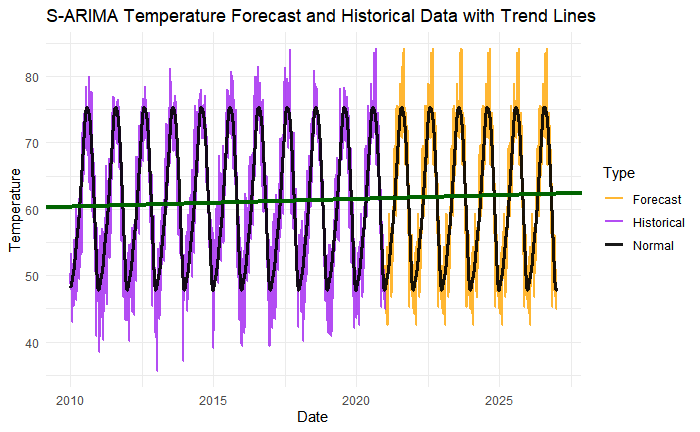
\includegraphics[width=.8\textwidth]{Final_Report/images/ARIMA_All_CA.png}
\vspace*{2mm}
\caption{S-ARIMA for all of California}
\end{figure}

\section{Conclusion \& Next Steps}
This research aimed to provide unique tools to individual consumers and small-scale farmers that would empower them to cultivate crops in a more effective manner. This research created a proof-of-concept that dynamically ingests weather data from across the United States and displays risks and recommendations for crop cultivation based on local micro-climates. Several next steps are outlined throughout the \textbf{\hyperref[sec:ma]{Models \& Analysis section}} and should be considered by researchers in the future. 

%%%%%%%%%%%%%%%%%%%%%%%%%%%%%%%%
%% ||| Section References ||| %%                           [B]
%%%%%%%%%%%%%%%%%%%%%%%%%%%%%%%%
%% Imported autoformating for References in the bib.bib file
%% References can be put into there and it should automatically format.  If issues we can build our own.

\bibliographystyle{johd}
\bibliography{bib}

%%%%%%%%%%%%%%%%%%%%%%%%%%%%%%%%

\appendix
\section{Appendix}
\subsection{Curated Data}
\label{sec:curated}
The following datasets were curated, stored in the \href{https://gtvault.sharepoint.com/:f:/s/MGT-6203Team95/Ev1dI-WU521EnSnFGUY9QigBHe4nMzpq5NIJo9s6VWLIoA?e=qEVO1C}{SharePoint repository}, and are ready for further analysis. 

\begin{itemize}[noitemsep]
    \item Crop Data by County, Mapped and Aggregated - California , 2010-2020
    \item 30-Year Normals by County, Mapped - California, 1991-2020
    \begin{itemize}[noitemsep]
        \item Average, Minimum, and Maximum Temperatures - Point Estimates and STD.DEVs
        \item Month-to-Date (MTD) Snow and Rain - Point Estimates
    \end{itemize}
    \item 30-Year Normals by Weather Station, Mapped - California, 1991-2020
    \item Daily Weather by County - California, 2010-2020
    \begin{itemize}[noitemsep]
        \item Dew Point
        \item Wind Gust / Max Wind Speed / 5 Min Wind Speed High
        \item Max Temp / Min Temp / Avg Temp
        \item Precipitation
        \item Elevation
        \item One-Hot Encoding for Basic Weather Event: Fog/Ran/Snow/Hail/Thunder/Tornado
    \end{itemize}
\end{itemize}

\subsection{Crop Choices}
\label{sec:choices}

This section describes the ten crops selected for observation in California. \\

\begin{tabularx}{1.0\textwidth} { 
  | >{\raggedright\arraybackslash}X 
  | >{\raggedright\arraybackslash}X | }
 \hline
 \textbf{California} \\
 \hline
 1. Rice \\
 2. Other Hay/Non Alfalfa \\
 3. Tomatoes \\
 4. Grapes \\
 5. Almonds \\
 6. Walnuts  \\
 7. Pistachios \\
 8. Oranges \\
 9. Strawberries \\
 10. Lettuce \\ 
\hline
\end{tabularx}

\end{document}